\documentclass[12pt]{article}

\usepackage[margin=0.6in]{geometry}
\setlength{\parindent}{0em}
\usepackage{mathtools}
\usepackage{amsmath}
\usepackage{array}
\usepackage{pgfplotstable}
\usepackage{pgfplots}
\usepackage{xcolor,colortbl}
\definecolor{Gray}{gray}{0.9}
\usepackage{tabularx}
\usepackage{bm}
\usepackage{graphicx}
\graphicspath{/Users/dotun/Dropbox/}

\begin{document}
\title{B503 Homework Assignment 5}
%\author{Oyedotun Oyesanmi}
\date{\today}
\maketitle



\textbf{2a \& b:}
\newcolumntype{g}{>{\columncolor{Gray}}}
\begin{table}[h]
	\begin{center}
		\begin{tabular}{| >{\centering\arraybackslash}m{4.186in} | g >{\centering\arraybackslash}m{2.842in}|}\hline
			
			\textbf{Table 1: Number of Object Comparisons} & \textbf{Table 2: Real Execution Time} \parbox{0pt}{\rule{0pt}{2ex+\baselineskip}}\\ 

		\end{tabular}\par\vskip-1.4pt
			\begin{tabular}{| >{\centering\arraybackslash}m{0.4in} | >{\centering\arraybackslash}m{0.8in} | >{\centering\arraybackslash}m{1in}     | >{\centering\arraybackslash}m{0.5in} | >{\centering\arraybackslash}m{0.8in} | g  >{\centering\arraybackslash}m{0.5in} | g >{\centering\arraybackslash}m{1in} | g  >{\centering\arraybackslash}m{1in} |}\hline
			
		\bm{$n$} & \bm{$Quicksort$} & \bm{$Badsort$} & \bm{$n^2$} & \bm{$nlog(n)$} & \bm{$n$} & \bm{$Quicksort$} & \bm{$Badsort$}  \parbox{0pt}{\rule{0pt}{2ex+\baselineskip}}\\ \hline
		10  & 53 & 100 & 100 & 33.2193 & 10000 & 0 & 274\parbox{0pt}{\rule{0pt}{3ex+\baselineskip}}\\  \hline
		20 & 148 &  769 & 400 & 86.4386 & 20000 & 0 & 2098\parbox{0pt}{\rule{0pt}{3ex+\baselineskip}}\\  \hline
		30 & 256 & 3058 & 900 & 147.207 & 25000 & 0 & 4511 \parbox{0pt}{\rule{0pt}{3ex+\baselineskip}}\\  \hline
		40 & 325 & 7603 & 1600 & 212.877 & 30000 & 0 & 9123\parbox{0pt}{\rule{0pt}{3ex+\baselineskip}}\\  \hline
		50 & 434 & 14875 & 2500 & 282.193 & 40000 & 0 & 37110 \parbox{0pt}{\rule{0pt}{3ex+\baselineskip}}\\  \hline
		60 & 543 & 21871 & 3600 & 354.413   \parbox{0pt}{\rule{0pt}{3ex+\baselineskip}}\\  \cline{1-5}
		70 & 688 & 40599 & 4900 & 429.05   \parbox{0pt}{\rule{0pt}{3ex+\baselineskip}}\\  \cline{1-5}
		80 & 869 & 55211 & 6400 & 505.754  \parbox{0pt}{\rule{0pt}{3ex+\baselineskip}}\\  \cline{1-5}
		90 & 933 & 73496 & 8100 & 584.267    \parbox{0pt}{\rule{0pt}{3ex+\baselineskip}}\\  \cline{1-5}
		100 & 1047 & 97603 & 10000 & 664.386  \parbox{0pt}{\rule{0pt}{3ex+\baselineskip}}\\  \cline{1-5}
		\end{tabular}
	\end{center}
\end{table}



\begin{figure}
	\textbf{2c:}
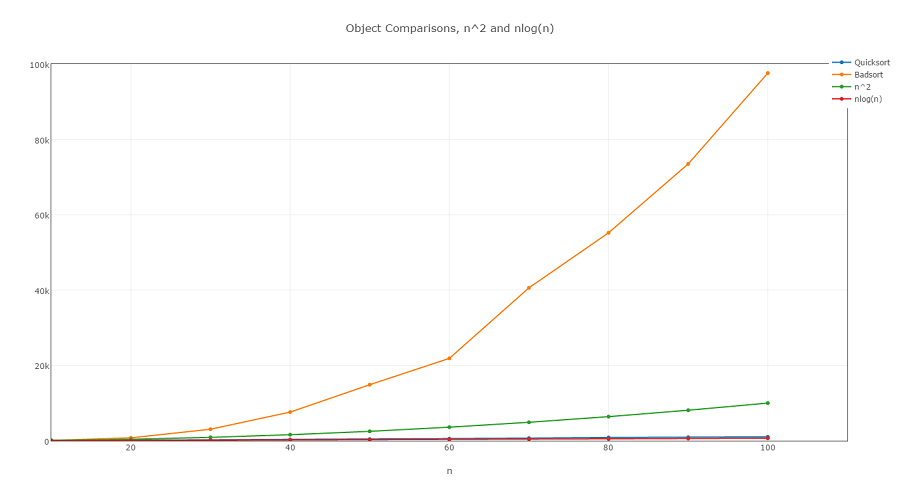
\includegraphics[scale=1.1,width=25cm,height=18cm,angle=90]{newplot.png}
\centering
\end{figure}

\pagebreak

\textbf{2d:}\\
Based on the reported comparisons, \texttt{badsort} makes more than double the number of comparisons compared to \texttt{quicksort}, in some instances, 20 times more comparisons.\\

Based on the reported execution times, \texttt{badsort} takes substantially longer time to execute than \texttt{quicksort}. In some instances, exponential time more than \texttt{quicksort}\\

\textbf{3a:}\\

\underline{Size of Stack Frame:}\\

For \texttt{badsort} to execute, it requires space for argument passed into it \texttt{int array} and \texttt{size of array}, then we need space for \texttt{index} variable declared within \texttt{badsort}.
Space is also required for multiple calls to \texttt{swap}, which in itself requires space for \texttt{int temp} and two integer arguments passed by reference.\\

\textbf{3b:}\\
\underline{Number of Stack Frames:}\\

One stack frame is required to call \texttt{badsort}, but, \texttt{badsort} itself makes several calls to \texttt{swap}. Calls to \texttt{swap} requires a stack frame, and the number of stack frames depends on the size of the array we are to sort and how randomly sorted the array is.\\

Therefore, since there is not a fixed number of  calls to \texttt{swap}, space complexity is not a fixed constant.\\

\underline{Asymptotic Upper Bond :}\\

Taking an arbitrary size of array, lets say \texttt{10}, running \texttt{badsort} on the same machine, the following comparisons was made by \texttt{badsort}:\\

\texttt{106, 174, 62, 128, 118, 104, 141, 123, 142, 102, 115, 129, 119, 86, 88}\\

we can conclude that the Upper bond for \texttt{badsort} should be not be greater than $O(n^2log(n))$\\

\underline{Asymptotic Lower Bond :}\\

Taking an arbitrary size of array, lets say \texttt{10}, running \texttt{badsort} on the same machine, the following comparisons was made by \texttt{badsort}:\\

\texttt{117, 127, 131, 116, 64, 91, 134, 149, 136, 98, 9}\\

we can conclude that the Lower bond for \texttt{badsort} should be not be greater than $\varTheta(log(n)^3)$\\

Therefore, we can conclude that, regardless the size of array input, comparison made by \texttt{badsort} will not be greater than $O(n^2log(n))$

\end{document}